\documentclass[12pt,a4paper]{article}
\usepackage[utf8]{inputenc}
\usepackage[T1]{fontenc}
\usepackage{amsmath,amssymb}
\usepackage{graphicx}
\usepackage{hyperref}
\usepackage{natbib}
\usepackage{booktabs}
\usepackage{geometry}
\usepackage{setspace}
\usepackage{authblk}

\geometry{margin=1in}
\onehalfspacing

\title{Beyond Pharmacologic Ferroptosis Inducers: Physical ROS Modalities for Drug-Tolerant Persister Cells}

\author[1]{Ezequiel Lares}
\affil[1]{Independent Researcher}

\date{}

\begin{document}

\maketitle

\begin{abstract}
Drug-tolerant persister cells that survive first-line cancer therapy are sensitized to ferroptosis --- an iron-dependent cell death pathway. The persister-ferroptosis field currently focuses exclusively on pharmacologic ferroptosis inducers (RSL3, erastin, GPX4 inhibitors) for clinical exploitation. Here we present a cross-literature analysis of 4,830 full-text cancer research articles (803 journals, 19 mechanisms, 22 cancer types, 2001-2026), alongside a separate archive of 5,584 abstract-only records, proposing that an entire class of physical ROS-generating modalities should be evaluated as spatially selective alternatives. Photodynamic therapy (PDT, 355 PubMed ferroptosis articles) and sonodynamic therapy (SDT, 121 PubMed ferroptosis articles) trigger ferroptosis through sensitizer-activated ROS generation, and additionally produce immunogenic cell death (ICD) --- a dual output that pharmacologic inducers have not been shown to reliably generate. PDT is established but depth-limited (light penetrates millimeters); SDT extends the same mechanism to deep-seated tumors via ultrasound (centimeters). We propose that physical modalities offer two advantages over systemic drugs for persister targeting: spatial selectivity (focused energy at the tumor, not systemic exposure) and ICD generation (potential immunotherapy synergy). This framing --- which connects two research communities that do not cite each other --- has not been systematically proposed. We present it as a research direction, not a validated strategy, and discuss extensively the PDT precedent (40 years without demonstrating robust ICD-immune synergy in randomized trials), the nanosonosensitizer confound, failed trials (CheckMate-498, BIND-014, Pexa-Vec), and the biological barriers that could prevent translation.
\end{abstract}

\textbf{Keywords:} drug-tolerant persisters, ferroptosis, photodynamic therapy, sonodynamic therapy, immunogenic cell death, physical modalities, ROS, spatially selective therapy, cross-literature analysis

\section{Introduction}

Cancer cells that survive first-line therapy --- drug-tolerant persister cells --- are a central obstacle to durable remission. Recent work has shown that these persisters are sensitized to ferroptosis, an iron-dependent cell death pathway driven by lethal lipid peroxidation \cite{higuchi2026_41481741}; \cite{berra2026_41872128}. This discovery has created urgent interest in finding clinically viable ferroptosis inducers. So far, the search has focused exclusively on pharmacologic agents: small-molecule inhibitors of GPX4 (the primary enzyme that repairs lipid peroxides) such as RSL3 and erastin \cite{lei2022_35338310}.

This article proposes that the search should be broadened. Photodynamic therapy (PDT) and sonodynamic therapy (SDT) --- physical modalities that use light or ultrasound to activate sensitizer molecules --- generate reactive oxygen species (ROS) that trigger the same ferroptosis pathway, with 355 and 121 PubMed-indexed ferroptosis articles, respectively. Unlike systemic drugs, these modalities deliver ROS locally to a defined tumor volume via focused energy, and they additionally produce immunogenic cell death (ICD) --- the release of molecular danger signals that can activate anti-tumor immune responses \cite{zhang2018_29575297}; \cite{ren2021_34646381}. Pharmacologic ferroptosis inducers have not been shown to reliably produce ICD.

The connection between the persister-ferroptosis field (which reads cancer biology journals) and the PDT/SDT-ferroptosis field (which reads materials chemistry and nanotechnology journals) has not been systematically made. These communities do not cite each other. This article bridges them.

We present a systematic analysis of 4,830 full-text cancer research articles spanning 19 therapeutic mechanisms and 22 cancer types (803 journals, 2001-2026), with a separate archive of 5,584 abstract-only records, a Monte Carlo biochemical simulation of ferroptosis sensitivity across cell phenotypes (16 million cells), and a specific, testable proposal: that physical ROS-generating modalities should be evaluated as spatially selective, ICD-generating alternatives to pharmacologic ferroptosis inducers for killing drug-tolerant persister cells. SDT specifically extends this approach to deep-seated tumors (pancreatic, hepatic, pelvic) that PDT cannot reach due to the limited tissue penetration of light.

\begin{figure}[ht]
\centering
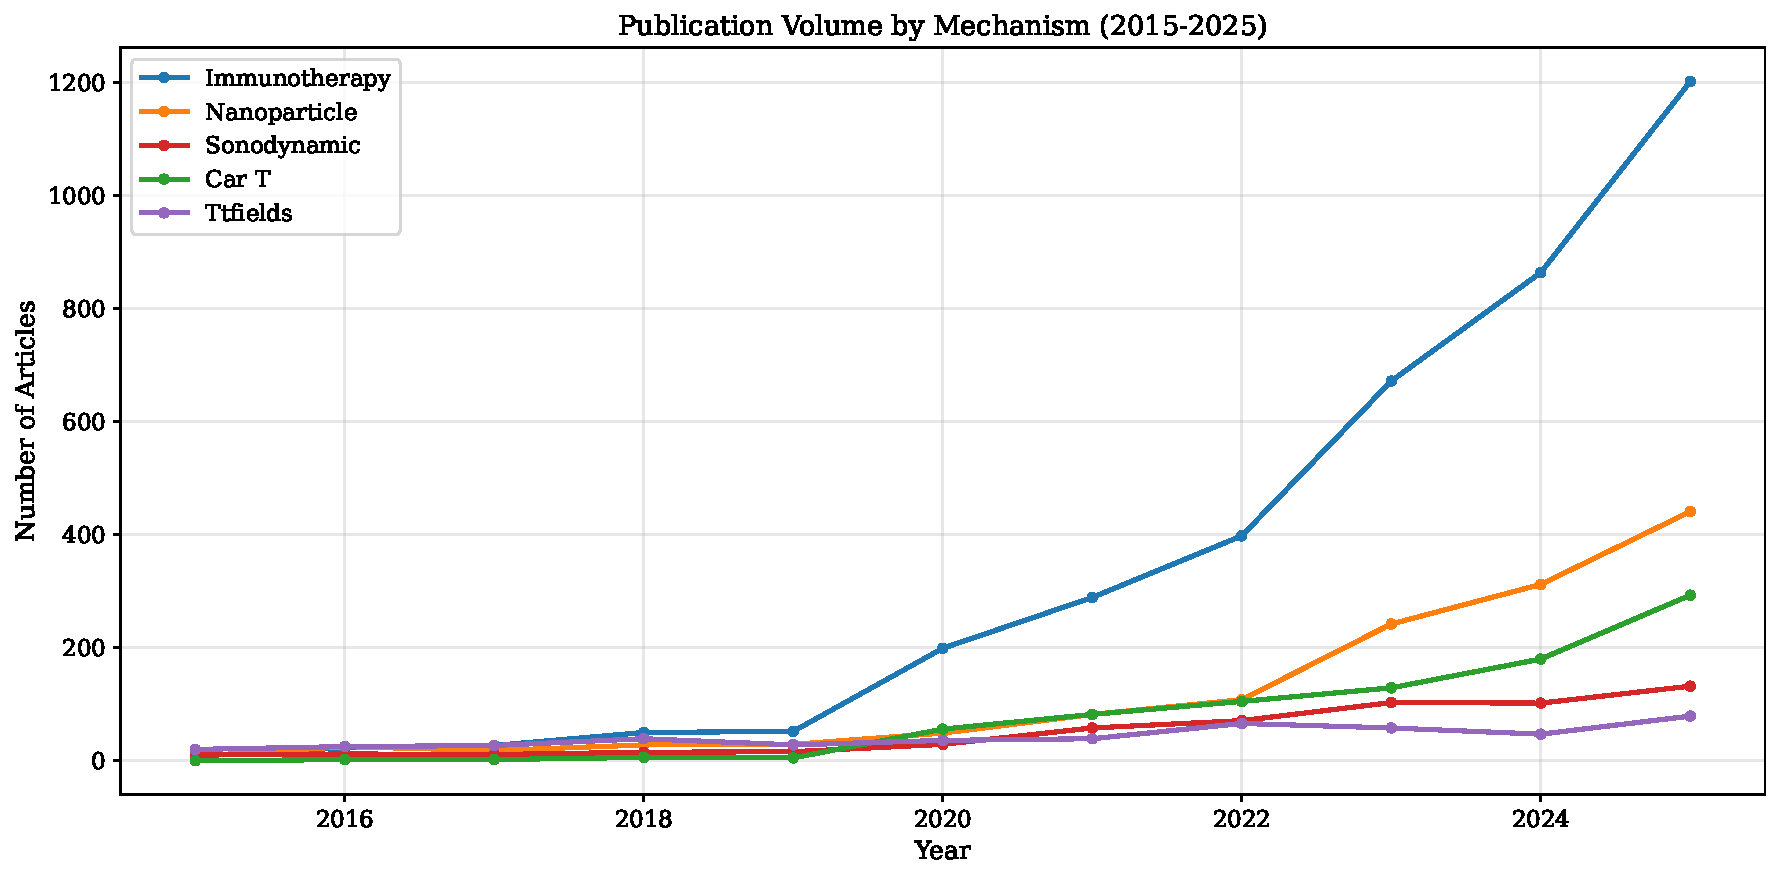
\includegraphics[width=\textwidth]{../figures/fig5_publication_trends.pdf}
\caption{Publication volume 2015--2025.}
\label{fig:fig5_publication_trends}
\end{figure}

\section{Methods}

\subsection{Search Strategy and Corpus Construction}

We conducted a systematic literature search of PubMed using the NCBI E-utilities API, covering publications indexed through March 2026. The search strategy employed 22 mechanism-specific query sets using established MeSH terms and free-text synonyms: for example, "tumor treating fields" OR "TTFields" OR "Optune" for TTFields; "chimeric antigen receptor" OR "CAR-T" OR "CAR T cell" for CAR-T therapy; "sonodynamic therapy" OR "sonosensitizer" for sonodynamic approaches. Results were enriched with metadata from OpenAlex (open access status, citation counts, topic classification) and PubMed Central or publisher-hosted OA URLs (full-text retrieval for open access articles).

\subsection{Inclusion and Exclusion Criteria}

Articles were included if they were returned by the PubMed search queries and addressed at least one of the 19 therapeutic mechanisms in the context of cancer treatment or cancer biology. No additional manual inclusion or exclusion filtering was applied beyond the search query constraints. The resulting archive therefore includes original research, clinical trial reports, systematic reviews, narrative reviews, and some case series. For quantitative analyses in this manuscript, we indexed only the 4,830 records for which local full text was available; the remaining 5,584 metadata/abstract-only records were retained in a separate archive and not used for the full-text-derived corpus statistics reported below. This distinction is important: article counts in the Results section refer to the full-text corpus unless explicitly stated otherwise.

\subsection{Categorization Framework}

Each article was tagged along three axes:

\textbf{Therapeutic mechanism(s):} Articles were assigned one or more of 19 tags representing distinct therapeutic modalities. We use "mechanism" broadly to encompass molecular targets (e.g., synthetic lethality), drug classes (e.g., ADCs), delivery platforms (e.g., nanoparticles), device-based interventions (e.g., TTFields), and biological strategies (e.g., microbiome modulation). This heterogeneous taxonomy reflects the diversity of the contemporary oncology toolkit; we prioritized practical distinctness over strict ontological consistency. The 19 tags are: (1) antibody-drug conjugate (ADC), (2) bioelectric modulation, (3) bispecific antibody, (4) CAR-T cell therapy, (5) CRISPR gene editing, (6) electrochemical therapy (including irreversible electroporation), (7) electrolysis, (8) epigenetic therapy, (9) frequency therapy (including pulsed electromagnetic fields), (10) high-intensity focused ultrasound (HIFU), (11) checkpoint immunotherapy, (12) mRNA cancer vaccine, (13) metabolic targeting, (14) microbiome modulation, (15) nanoparticle delivery, (16) oncolytic virotherapy, (17) sonodynamic therapy, (18) synthetic lethality, and (19) tumor-treating fields (TTFields). Articles addressing multiple mechanisms received multiple tags, enabling convergence analysis.

\textbf{Cancer type(s):} Articles were assigned to one or more of 22 cancer types: bladder, breast, cervical, colorectal, esophageal, gastric, glioblastoma, head-and-neck, kidney, leukemia, liver, lung, lymphoma, melanoma, mesothelioma, myeloma, neuroblastoma, ovarian, pancreatic, prostate, sarcoma, and thyroid.

\textbf{Evidence level:} Articles were classified into one of six tiers: (1) Phase III clinical trial or randomized controlled trial, (2) Phase II clinical trial, (3) Phase I clinical trial, (4) preclinical in vivo, (5) preclinical in vitro, or (6) theoretical/computational/review. Classification was based on the highest level of evidence reported or reviewed in each article.

\subsection{Analytical Approach}

Four primary analyses were conducted:

\textit{Mechanism-cancer matrix:} A 19 x 22 cross-tabulation of article counts by mechanism and cancer type, identifying concentration patterns and gaps.

\textit{Convergence map:} Identification and quantification of all mechanism-pair co-occurrences across the corpus, revealing which multi-mechanism combinations are most actively researched.

\textit{Evidence-tier analysis:} Assessment of the highest clinical evidence level achieved for each mechanism, identifying translational bottlenecks.

\textit{Gap analysis:} Identification of mechanism-cancer and mechanism-mechanism pairs with zero or near-zero co-occurrence in our corpus, noting that some gaps reflect search query design rather than genuine research absence.

Impact metrics (citation counts, iCite Relative Citation Ratio) were used to identify landmark publications and assess field-normalized influence. Publication volume was tracked annually to identify growth trajectories.

\subsection{Limitations}

Several limitations should be acknowledged. First, all tagging was performed by automated keyword matching against curated dictionaries (no manual article-level review), introducing potential misclassification. Short or ambiguous terms may generate false positives, and articles using non-standard terminology may be missed. Second, the archive was constructed from PubMed queries only and does not capture every relevant publication, particularly articles in non-English languages, preprints not yet indexed in PubMed, or studies using unconventional terminology for established mechanisms. Third, the quantitative corpus analyzed here is restricted to the 4,830 records with local full text; although this improves traceability and reproducibility, it also excludes 5,584 abstract-only records that may materially change article-count-based field comparisons. Fourth, evidence-level classification was based on keyword detection (e.g., "phase 3", "in vivo") rather than independent trial registry verification; importantly, only 42\% of the full-text corpus (n = 2,037) received an evidence-level tag, meaning that most articles have unclassified evidence levels. Claims about the absence of clinical trials for specific mechanisms should therefore be interpreted as "not detected in our keyword-based analysis" rather than definitive statements. Fifth, multi-mechanism co-occurrence counts reflect articles tagged with multiple mechanism keywords, which includes both intentional combination studies and reviews that discuss multiple mechanisms without testing them in combination. The true rate of experimental multi-mechanism studies is likely lower. Sixth, the 19-mechanism taxonomy has not been tested for sensitivity: collapsing the 7 physical/energy categories into 2-3 broader groups (physical ablation, bioelectric modulation, field-based therapy) would reduce the number of "zero publication gaps" and could change the gap analysis conclusions. Our findings should be interpreted as taxonomy-dependent until sensitivity analyses with alternative groupings are performed. Finally, article counts serve as a proxy for research intensity but do not directly measure quality, reproducibility, or clinical significance, and the corpus inherits any publication biases present in the indexed literature.

\section{Results}

\subsection{Corpus Overview}

The final full-text corpus comprised 4,830 articles from 803 journals, with impact metrics available for 3,739 articles via iCite. Publication volume increased 31-fold over the study period, from 38 full-text articles in 2015 to 1,167 in 2025, with 186 articles already indexed in the first quarter of 2026. Growth was non-linear, with a marked inflection point in 2020 (257 full-text articles, a 2.4-fold increase over 2019's 106 articles), coinciding with the maturation of mRNA technology catalyzed by COVID-19 vaccine development and the broadening clinical experience with checkpoint immunotherapy.

\begin{figure}[ht]
\centering
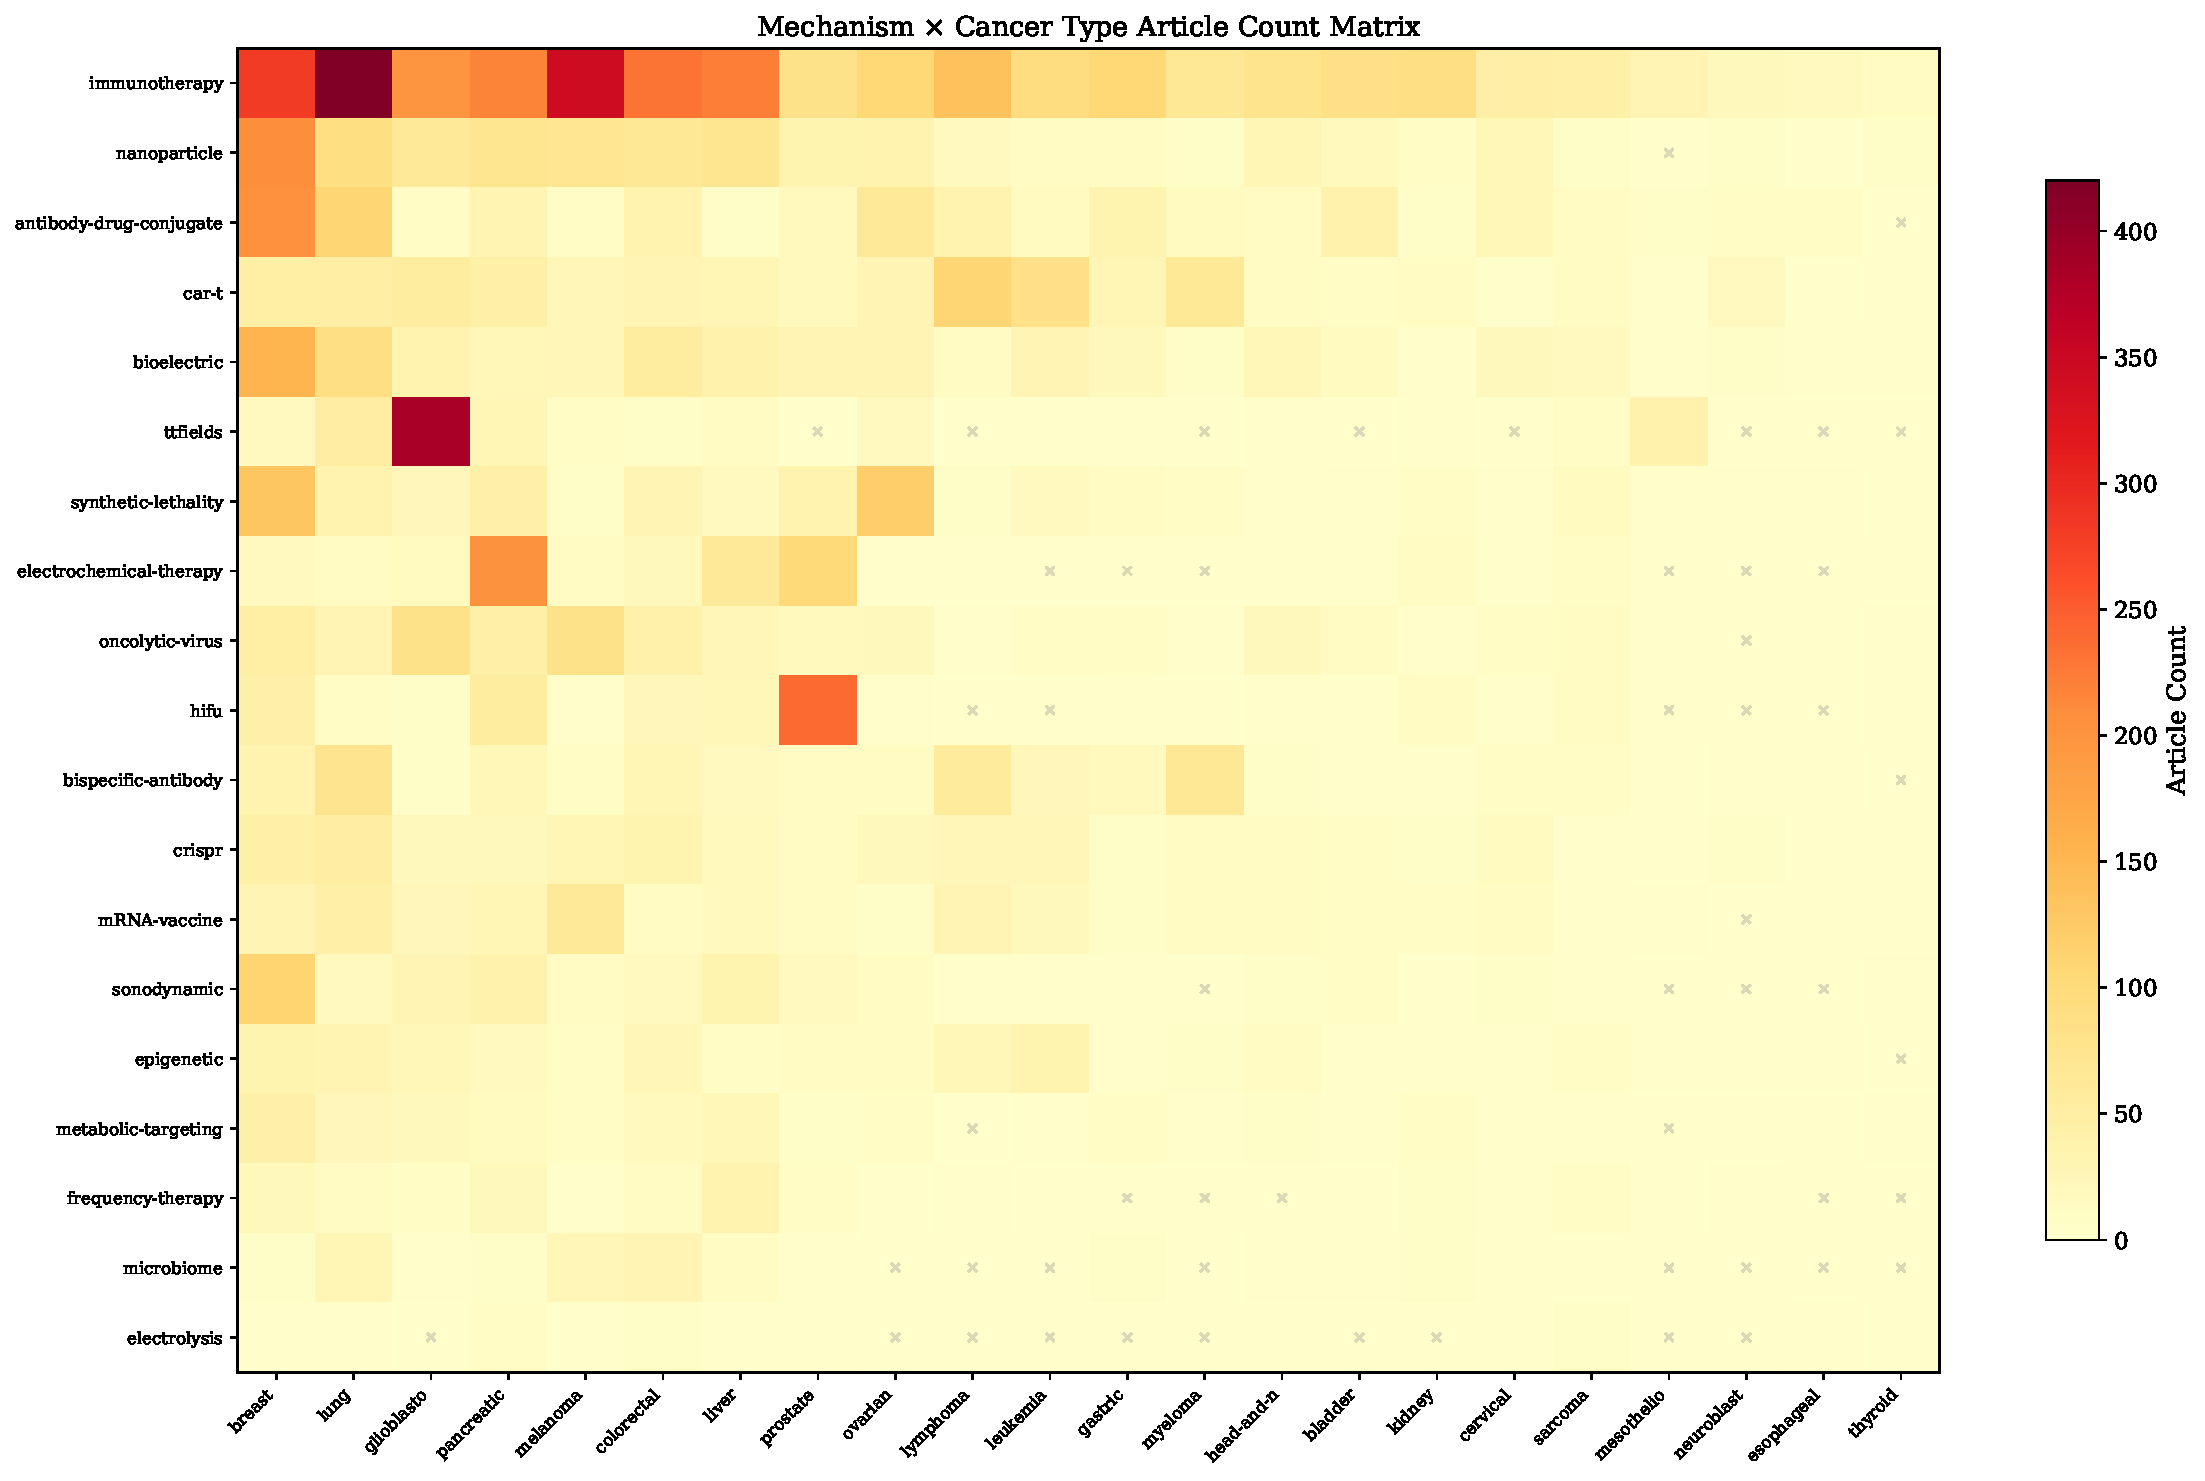
\includegraphics[width=\textwidth]{../figures/fig2_mechanism_heatmap.pdf}
\caption{Mechanism $\times$ cancer type matrix.}
\label{fig:fig2_mechanism_heatmap}
\end{figure}

The fastest-growing mechanisms by absolute article count between 2020 and 2025 were immunotherapy (+504\% annual articles), nanoparticle delivery (+800\%), CAR-T therapy (+423\%), and sonodynamic therapy (+355\%). These growth rates reflect both the maturation of established approaches and the emergence of new platform technologies.

\subsection{Physical and Energy-Based Mechanisms}

\subsubsection{Tumor-Treating Fields (TTFields)}

TTFields, which deliver low-intensity (1-3 V/cm), intermediate-frequency (100-300 kHz) alternating electric fields to disrupt mitotic spindle formation and organelle assembly in dividing cells \cite{rominiyi2021_33144698}, represent the most clinically advanced physical therapy mechanism in our corpus. We identified 502 TTFields-tagged articles across 14 of 22 cancer types (575 total cross-tabulation instances in the mechanism-cancer matrix, reflecting articles tagged with multiple cancer types). The evidence-level analysis identified 73 articles classified at the Phase III tier; however, this count includes reviews and meta-analyses that discuss Phase III trial results (e.g., the EF-14 trial) in addition to primary Phase III trial reports. The true number of distinct Phase III TTFields trial publications is substantially smaller, though still the second-highest of any mechanism after checkpoint immunotherapy.

The evidence base is anchored by the EF-14 trial, a pivotal Phase III randomized clinical trial demonstrating that TTFields plus maintenance temozolomide significantly improved median overall survival (20.9 vs. 16.0 months, p < 0.001) and 5-year survival (13\% vs. 5\%) in newly diagnosed glioblastoma \cite{stupp2017_29260225}. This trial, with 2,494 citations, is the fifth-highest-impact article in our entire corpus (RCR 69.5, 100th percentile). An earlier randomized trial \cite{stupp2015_26670971} (1,203 citations) established the foundation for FDA approval of the Optune device.

Beyond glioblastoma, TTFields are being investigated in mesothelioma (38 articles), lung cancer (51 articles), pancreatic cancer (27 articles), and ovarian cancer (15 articles). The LUNAR Phase III trial demonstrated improved overall survival in metastatic non-small-cell lung cancer (NSCLC) when TTFields were added to standard systemic therapy \cite{leal2023_37657460}. A comprehensive review characterizes TTFields as a distinct fourth modality of cancer treatment alongside surgery, radiation, and pharmacotherapy \cite{rominiyi2021_33144698}.

TTFields have zero or near-zero publications in prostate cancer, lymphoma, myeloma, bladder cancer, and cervical cancer in our corpus, though some of these gaps may reflect search query design rather than genuine absence.

\subsubsection{High-Intensity Focused Ultrasound (HIFU)}

HIFU uses convergent acoustic energy to achieve thermal ablation of tumor tissue at a defined focal point without incision. Our full-text corpus contains 81 HIFU articles across 12 cancer types. The dominant application is prostate cancer (29 full-text articles), where HIFU is established as a focal therapy option \cite{maloney2015_25367011}; \cite{guillaumier2018_29960750}. Notably, a multicentric study reported 5-year outcomes of focal HIFU for clinically significant nonmetastatic prostate cancer \cite{guillaumier2018_29960750} (309 citations), demonstrating favorable oncologic control with preserved quality of life.

HIFU research in breast cancer (42 articles), pancreatic cancer (50 articles), and liver cancer (22 articles) is expanding. A systematic review positions HIFU alongside radiofrequency ablation, microwave ablation, and cryoablation as viable alternatives to surgical resection for small tumors \cite{van2021_33840627}.

\subsubsection{Sonodynamic Therapy}

Sonodynamic therapy (SDT) exploits low-intensity ultrasound to activate sonosensitizer molecules that generate reactive oxygen species (ROS) within tumor tissue. Our full-text corpus contains 189 SDT articles across 15 cancer types, making it one of the most actively researched physical modalities in the energy-based subset. However, SDT faces significant translational challenges. Our keyword-based evidence classification detected only 1 Phase I article in the full-text corpus, with the balance of the literature remaining heavily preclinical. Independent PubMed verification using broader clinical terms identifies substantially more SDT-related records at the abstract level, suggesting more early-phase clinical activity than our full-text corpus captures. Nonetheless, no large randomized Phase 2 or Phase 3 trial of SDT has been reported in a major oncology journal, and SDT remains overwhelmingly a preclinical field in terms of rigorous clinical evidence.

The preclinical literature is large and growing. Landmark studies have demonstrated nanoenzyme-augmented SDT with catalytic tumor oxygenation \cite{zhu2018_29613770} (571 citations), graphene-augmented sonocatalytic tumor eradication \cite{dai2017_28829584} (300 citations), and piezotronic effect-augmented sonosensitizers \cite{zhao2022_35699224} (218 citations). The convergence of SDT with nanoparticle delivery is particularly active (267 combined articles), and SDT-immunotherapy combinations are growing rapidly (105 articles), with emerging evidence for SDT-based immunogenic cell death \cite{xu2021_33122099}; \cite{yang2023_36437106}.

A distinctive molecular signature emerges from our full-text corpus analysis that sets SDT apart from all other physical modalities. SDT uniquely and potently engages the \textbf{ferroptosis} pathway --- iron-dependent, lipid peroxidation-mediated cell death --- with 36 full-text articles linking SDT to ferroptosis, compared to 0 for TTFields, 1 for HIFU, and 3 for IRE. More specifically, 79 SDT full-text articles (42\% of the SDT corpus) mention the glutathione/GPX4 axis, underscoring how centrally redox buffering appears in this literature. The proposed causal chain --- ultrasound-activated ROS generation $\rightarrow$ glutathione depletion $\rightarrow$ GPX4 inactivation $\rightarrow$ lipid peroxidation $\rightarrow$ ferroptosis $\rightarrow$ DAMP release $\rightarrow$ immunogenic cell death --- is supported at each individual link by published preclinical data \cite{xiong2021_34027953}; \cite{xu2021_33408790}; \cite{dong2021_34655115}; \cite{zhang2018_29575297}. We discuss the implications of this pattern in Section 4.4.

The primary barriers to clinical translation include the lack of standardized sonosensitizer formulations approved for human use, the absence of validated ultrasound dosimetry protocols for SDT (as distinct from diagnostic or HIFU applications), and the challenge of demonstrating SDT superiority or complementarity to established modalities in registrational trials. Breast cancer is the most studied SDT target in the full-text corpus (42 articles), followed by liver cancer (19 articles) and pancreatic cancer (12 articles).

\subsubsection{Frequency Therapy and Electrolysis}

Frequency therapy --- encompassing pulsed electromagnetic fields (PEMF), radiofrequency ablation in immunomodulatory contexts, and resonance-based approaches --- is represented by 97 full-text articles across 11 cancer types. This is a nascent field with mechanistic diversity that complicates systematic evaluation. A foundational review \cite{vadala2016_27748048} (113 citations) described mechanisms of PEMF in oncology, including disruption of mitotic spindle formation, induction of apoptosis, and immunomodulatory effects.

Electrolysis as a direct antitumor mechanism is the smallest category in our full-text corpus (11 articles across only a handful of cancer contexts), but includes innovative work on amorphous liquid metal electrodes for conformable electrochemical tumor therapy \cite{sun2017_28918265} (114 citations) and platinum nanoparticle-enabled electrodynamic therapy \cite{gu2019_30734370} (211 citations).

\subsubsection{Electrochemical Therapy}

Electrochemical therapy (EChT), dominated by irreversible electroporation (IRE), is represented by 185 full-text articles across 14 cancer types. Pancreatic cancer (61 articles) and prostate cancer (30 articles) are the primary applications. A foundational paper introduced the concept of tissue ablation through irreversible electroporation \cite{davalos2005_15771276} (1,241 citations), and subsequent clinical development has demonstrated safety and feasibility in locally advanced pancreatic cancer \cite{martin2015_26258317} (400 citations) and localized prostate cancer \cite{scheltema2016_27150293}; \cite{scheltema2018_29594551}.

A pivotal development is the combination of IRE with immunotherapy: high-frequency IRE has been shown to induce immunogenic cell death \cite{unknown2019_31130474} (168 citations), and emerging data demonstrate synergy between IRE and checkpoint blockade plus TLR7 stimulation \cite{narayanan2019_31409607} (111 citations). The IRE-immunotherapy convergence (45 articles) represents a growing axis of investigation. However, lymphoma, leukemia, gastric cancer, and myeloma have zero EChT publications despite established clinical experience in other solid tumors.

\subsection{Bioelectric Modulation}

Bioelectric research encompasses membrane potential manipulation, ion channel modulation, voltage-gated signaling in cancer biology, and electroporation-based drug delivery. Our full-text corpus contains 253 articles across 19 cancer types, with broad conceptual range but limited direct clinical antitumor translation.

A landmark Cell paper established the conceptual framework for bioelectric signaling as a reprogrammable circuit underlying embryogenesis, regeneration, and cancer \cite{levin2021_33826908} (463 citations), arguing that endogenous bioelectric patterns constitute an informational layer that can be therapeutically manipulated. Earlier work on endogenous voltage gradients controlling growth and form \cite{levin2017_28633567} (289 citations) provided the biophysical foundation. The identification that mitochondrial membrane potential marks cells with enhanced stemness \cite{sukumar2016_26674251} (370 citations) has implications for targeting cancer stem cell populations.

Despite this conceptual richness, translational progress toward direct antitumor bioelectric interventions has been limited. While 3 articles in our corpus were tagged as Phase III under the bioelectric category, manual review reveals these address supportive care outcomes rather than bioelectric antitumor therapy. No Phase II or Phase III trial of a direct bioelectric antitumor intervention was identified.

\subsection{Immune-Based Approaches}

\subsubsection{Checkpoint Immunotherapy}

Checkpoint immunotherapy is the dominant mechanism in our full-text corpus, with 2,302 articles across all 22 cancer types. This reflects its established clinical role across multiple tumor types. The highest concentrations are in lung cancer (250 articles), melanoma (207 articles), breast cancer (162 articles), pancreatic cancer (138 articles), colorectal cancer (136 articles), liver cancer (133 articles), and glioblastoma (117 articles).

Key landmark articles include a comprehensive review of PD-1/PD-L1 and CTLA-4 checkpoint inhibitors \cite{shiravand2022_35621637} (1,191 citations), the comprehensive management review establishing temozolomide plus TTFields as the standard of care in glioblastoma and surveying immunotherapy as a promising but significantly challenged area due to the blood-brain barrier and unique immune microenvironment \cite{tan2020_32478924} (1,989 citations), and combination immunotherapy for hepatocellular carcinoma reviewing how approximately 30\% of HCC exhibits intrinsic resistance to single-agent ICIs and how combination strategies (anti-PD-1/PD-L1 with anti-angiogenics or dual checkpoint blockade) have improved first-line outcomes \cite{rimassa2023_36933770} (310 citations). STAT3 targeting as a convergence point for oncogenic signaling and immunomodulation has been extensively reviewed \cite{zou2020_32972405} (1,011 citations).

The most active convergence axes for immunotherapy in the full-text corpus include combinations with CAR-T (417 articles), oncolytic viruses (262 articles), nanoparticle delivery (193 articles), mRNA vaccines (172 articles), CRISPR (167 articles), bispecific antibodies (139 articles), metabolic targeting (127 articles), microbiome modulation (100 articles), ADCs (78 articles), SDT (53 articles), and TTFields (47 articles). Immunotherapy remains the central hub of the convergence network.

\subsubsection{CAR-T Cell Therapy}

CAR-T therapy is represented by 474 full-text articles across all 22 cancer types. The literature has evolved from early hematologic successes in B-cell leukemia and lymphoma \cite{rafiq2020_31848460} (1,400 citations) toward aggressive expansion into solid tumors.

Key developments include: IL-15-armored GPC3-targeted CAR-T cells for solid cancers \cite{steffin2025_39604730} (170 citations), representing a next-generation approach to overcoming the immunosuppressive tumor microenvironment; Claudin18.2-specific CAR-T cells showing promising Phase I results in gastrointestinal cancers \cite{qi2022_35534566} (546 citations); and IL-10-expressing CAR-T cells that resist dysfunction and mediate durable clearance of solid tumors \cite{zhao2024_38168996} (228 citations), demonstrating that cytokine engineering of CAR-T cells can overcome exhaustion.

CRISPR-based engineering of CAR-T cells is a rapidly growing convergence axis (95 full-text articles), exemplified by RASA2 ablation enhancing antigen sensitivity \cite{carnevale2022_36002574} (207 citations) and adenosine A2A receptor deletion enhancing efficacy \cite{giuffrida2021_34050151} (199 citations). The allogeneic CRISPR-Cas9-engineered CAR-T therapy CTX130, targeting CD70 in T-cell lymphoma, has demonstrated safety in Phase I \cite{iyer2025_39617017} (58 citations), representing a milestone for gene-edited cell therapies. CAR-T combined with oncolytic viruses (40 articles) and bispecific antibodies (30 articles) represents additional emerging convergence zones.

\subsubsection{Bispecific Antibodies}

Bispecific antibodies, engineered to simultaneously bind two distinct targets (typically a tumor antigen and an immune effector molecule), are represented by 248 full-text articles across 20 of 22 cancer types. Myeloma is a particularly active area (22 articles), with real-world data on teclistamab demonstrating clinical utility in relapsed/refractory disease \cite{riedhammer2024_38245601} (94 citations). Lung cancer applications are expanding, with KN046, a PD-L1/CTLA-4 bispecific, showing Phase II results in combination with chemotherapy for first-line metastatic NSCLC \cite{zhao2024_38508135} (38 citations), and the EGFRxHER3 bispecific izalontamab reporting first-in-human results \cite{xue2025_40260627}.

Bispecific antibody convergence with ADCs (42 articles) is an active area combining target engagement with cytotoxic payload delivery.

\subsubsection{mRNA Cancer Vaccines}

mRNA cancer vaccines represent one of the most dynamic areas in the full-text corpus: 341 articles across 20 cancer types. The field was catalyzed by the COVID-19 mRNA vaccine platform, which demonstrated the feasibility of rapid, scalable mRNA production and lipid nanoparticle delivery \cite{szabo2022_35189345} (279 citations). A comprehensive Lancet Oncology review established the clinical landscape \cite{lorentzen2022_36174631} (470 citations), documenting over 120 ongoing clinical trials.

The landmark article in this category is the Nature report on personalized RNA neoantigen vaccines stimulating T-cell responses in pancreatic ductal adenocarcinoma \cite{rojas2023_37165196} (1,153 citations, RCR 90.3, 100th percentile) ---the second-highest-impact article in our entire corpus. This Phase I trial of autogene cevumeran, an individualized neoantigen vaccine based on uridine mRNA-lipoplex nanoparticles, demonstrated that personalized vaccination could elicit measurable T-cell responses against patient-specific neoantigens in one of the most treatment-resistant cancers.

The mRNA vaccine field intersects strongly with immunotherapy (172 articles) and nanoparticle delivery (73 articles), reflecting the inherent dependence of mRNA vaccines on both immune activation and delivery technology. A recent clinical advances review documents the current pipeline across melanoma, glioblastoma, lung, breast, and prostate cancers \cite{yaremenko2025_39798545} (74 citations). Lipid nanoparticle-mediated lymph node-targeting delivery of mRNA cancer vaccines has been shown to elicit robust CD8+ T-cell responses \cite{chen2022_35969778} (371 citations).

\subsubsection{Oncolytic Viruses}

Oncolytic virotherapy is represented by 378 full-text articles across 19 cancer types. Glioblastoma is the most studied target (43 articles), followed by melanoma (51 articles), where T-VEC (talimogene laherparepvec) established the precedent for oncolytic virus approval. A comprehensive Nature Reviews Clinical Oncology review characterizes the field's progress and challenges \cite{shalhout2023_36631681} (489 citations), noting that oncolytic viruses offer selective replication in tumor cells, delivery of multiple transgene payloads, induction of immunogenic cell death, and promotion of antitumor immunity.

A notable 2025 Cell paper reported a hyperacute rejection-engineered oncolytic virus designed for interventional clinical trials in refractory cancer patients \cite{zhong2025_39826543} (67 citations), addressing the critical limitations of intravenous safety and inherent immune neutralization. In hepatocellular carcinoma, the oncolytic virus VG161 showed activity in a Nature-published Phase I study \cite{shen2025_40108464} (53 citations). The emerging field of OV-based cancer immunotherapy has been comprehensively reviewed in Trends in Cancer \cite{ma2023_36402738} (264 citations), positioning oncolytic viruses as multi-faceted tumor killers that combine direct lysis with immune potentiation.

The strongest convergence axis is oncolytic virus-immunotherapy (262 full-text articles), consistent with the mechanistic rationale that viral oncolysis generates immunogenic cell death that may synergize with checkpoint blockade \cite{shalhout2023_36631681}; \cite{ma2023_36402738}. Combinations with CAR-T (40 articles) and nanoparticle delivery remain emergent.

\subsection{Precision Molecular Approaches}

\subsubsection{CRISPR Gene Editing}

CRISPR-based approaches are represented by 336 full-text articles across 20 cancer types, with no Phase II or Phase III articles detected by our automated classification, placing CRISPR among the most preclinical-heavy mechanisms in our analysis. Despite this, the conceptual impact is enormous: CRISPR screens have defined unified hallmarks of cancer cell-autonomous immune evasion, providing a systematic map of therapeutic targets \cite{huber2026_41417728}.

Key convergence axes include CRISPR-immunotherapy (167 articles), CRISPR-CAR-T (95 articles), CRISPR-synthetic lethality (50 articles), and CRISPR-nanoparticle (29 articles). The engineering of next-generation CAR-T cells with CRISPR-Cas9 has been extensively reviewed \cite{dimitri2022_35303871} (314 citations), and clinical milestones include non-viral precision T-cell receptor replacement for personalized cell therapy \cite{foy2023_36356599} (256 citations) and the COBALT-LYM Phase I trial of CRISPR-edited allogeneic CAR-T for T-cell lymphoma \cite{iyer2025_39617017} (58 citations).

Precision nanomedicine integrating CRISPR with nanoparticle delivery for tumor microenvironment modulation represents a growing area \cite{sabit2025_40457437} (101 citations).

\subsubsection{Synthetic Lethality}

Synthetic lethality --- the paradigm in which loss of two genes is lethal while loss of either alone is viable ---is represented by 370 full-text articles across 21 cancer types. PARP inhibitors, the clinical embodiment of this concept, have achieved broad clinical use in breast cancer (69 articles), ovarian cancer (73 articles), pancreatic cancer (25 articles), and prostate cancer (24 articles). A pan-tumor review documented the expanding role of PARP inhibitors across multiple malignancies \cite{hage2025_39791278} (21 citations).

The concept of synthetic lethality as an engine for cancer drug target discovery has been comprehensively reviewed \cite{huang2020_31712683} (458 citations), and CRISPR-synthetic lethality combinations (63 articles) represent a powerful approach for systematic identification of new synthetic lethal pairs. Transcription-replication conflicts have been identified as a mechanistic basis for PARP inhibitor sensitivity \cite{petropoulos2024_38509368} (160 citations), expanding the theoretical framework beyond BRCA mutations.

Our corpus detected zero synthetic lethality-myeloma co-tagged articles; however, independent PubMed verification reveals at least 11 publications on PARP inhibitors in multiple myeloma, including early-phase clinical data on veliparib combined with bortezomib. This gap is therefore an artifact of our search query design rather than a genuine absence of research. The myeloma-PARP axis is under-researched relative to breast or ovarian cancer applications, but it is not unexplored.

\subsubsection{Antibody-Drug Conjugates (ADCs)}

ADCs are represented by 285 full-text articles across 21 cancer types. The field is dominated by breast cancer applications (92 articles), lung cancer (48 articles), and ovarian cancer (29 articles). The changing treatment landscape of EGFR-mutant NSCLC has been shaped by ADC development alongside bispecific antibodies \cite{zhou2025_39614090} (106 citations).

ADC convergence with immunotherapy (160 articles) is well established, and combinations with CAR-T (42 articles) and bispecific antibodies (42 articles) are emerging.

\subsubsection{Epigenetic Therapy}

Epigenetic approaches (DNA methylation inhibitors, histone deacetylase inhibitors, bromodomain inhibitors, and related agents) are represented by 184 full-text articles across 20 cancer types. A landmark Cell Death Discovery review established the current state of clinical translation \cite{yu2024_38225241} (223 citations), and a Signal Transduction and Targeted Therapy paper provided a comprehensive framework for epigenetic regulation in the tumor microenvironment \cite{yang2023_37217462} (322 citations).

The most impactful single finding in this category is the Nature paper demonstrating that NBS1 lactylation is required for efficient DNA repair and chemotherapy resistance \cite{chen2024_38961290} (413 citations, RCR 56.2), linking metabolic reprogramming (the Warburg effect) to epigenetic modification of the DNA damage response. This exemplifies how mechanistic convergence at the molecular level can reveal new therapeutic vulnerabilities.

Epigenetic-immunotherapy convergence (78 articles) is the dominant combination.

\subsection{Delivery and Microenvironment}

\subsubsection{Nanoparticle Delivery}

Nanoparticle-based delivery systems constitute the second-largest mechanism category in our full-text corpus: 522 articles across 20 cancer types. An important distinction must be drawn between established and experimental nanoplatforms. Several nanomedicines have achieved FDA approval, including liposomal doxorubicin (Doxil, 1995), nab-paclitaxel (Abraxane, 2005), liposomal irinotecan (Onivyde, 2015), and liposomal daunorubicin-cytarabine (Vyxeos, 2017) \cite{fulton2023_37047585}. These approved nanomedicines are typically described by drug name rather than "nanoparticle" in the literature and are therefore underrepresented in our corpus. The translational gap identified here primarily applies to novel experimental nanoplatforms --- metal, polymer, and inorganic nanoparticles --- which remain overwhelmingly preclinical in our full-text corpus. This distinction between proven liposomal/albumin-bound formulations and the broader experimental nanoparticle literature is critical: the former demonstrate that nanomedicine can succeed clinically, while the latter face substantial barriers to replicating that success.

The nanoparticle literature spans gold, silver, and iron oxide nanoparticles \cite{singh2025_39501968} (88 citations), liposomal formulations \cite{fulton2023_37047585} (215 citations), lipid nanoparticles for mRNA delivery \cite{chen2022_35969778} (371 citations), and precision nanomedicine for tumor microenvironment modulation \cite{sabit2025_40457437} (101 citations). The convergence with immunotherapy (193 articles) and sonodynamic therapy (118 articles) is extensive, as nanoparticles serve as both therapeutic agents and delivery vehicles for other modalities.

The fundamental translational barriers include: (a) heterogeneous nanoparticle pharmacokinetics and biodistribution that are difficult to predict from preclinical models; (b) manufacturing scalability and reproducibility challenges; (c) regulatory uncertainty around the classification and approval pathway for nanoparticle-drug combinations; and (d) the enhanced permeability and retention (EPR) effect, which is robust in rodent tumors but inconsistent in human cancers. Breast cancer (172 articles), lung cancer (76 articles), and liver cancer (66 articles) are the primary targets. Mesothelioma has zero nanoparticle publications despite the appeal of local delivery to pleural surfaces.

\subsubsection{Metabolic Targeting}

Metabolic targeting --- exploitation of altered cancer cell metabolism, particularly the Warburg effect, glutamine addiction, and lipid metabolism dependencies ---is represented by 277 full-text articles across 20 cancer types. A comprehensive Nature Reviews Drug Discovery article \cite{stine2022_34862480} (1,127 citations) chronicles the hundred-year journey from Warburg's discovery to contemporary precision metabolic oncology.

The convergence of metabolic targeting with immunotherapy (127 articles) reflects the recognition that metabolic reprogramming of the tumor microenvironment suppresses immune function and that metabolic interventions can restore immunocompetence. The landmark demonstration that glycolysis modulation can enhance checkpoint immunotherapy \cite{chelakkot2023_36768924} (341 citations) illustrates this principle. Glutamine addiction as a therapeutic target was comprehensively reviewed in a highly cited Trends in Biochemical Sciences paper \cite{wise2010_20570523} (1,747 citations).

Metabolic targeting has limited representation in lymphoma within our corpus, though broader PubMed searches suggest this gap partly reflects our search query design.

\subsubsection{Microbiome Modulation}

Microbiome modulation is the most recently emergent mechanism in our analysis: 109 full-text articles across 11 cancer types. The field has been catalyzed by the recognition that gut microbiota composition influences checkpoint immunotherapy response, as comprehensively reviewed in Nature Reviews Cancer \cite{fernandes2022_36253536} (258 citations) and Nature Medicine \cite{park2022_35440726} (467 citations).

Fecal microbiota transplantation (FMT) combined with checkpoint inhibitors has emerged as a clinical strategy, with a Gut Microbes review characterizing optimization approaches \cite{lin2025_39826104} (56 citations) and a meta-analysis evaluating FMT-ICI combinations \cite{lin2025_40484955} (23 citations). The DIET randomized trial investigated dietary intervention to modulate microbiome composition in melanoma patients receiving immunotherapy \cite{farias2024_39633321} (21 citations).

Microbiome-immunotherapy convergence (100 articles) dominates the microbiome literature in our corpus.

\subsection{Cross-Mechanism Convergence: Where Synergies Emerge}

Of the 4,830 articles in our full-text corpus, 1,985 (41\%) are tagged with two or more therapeutic mechanism keywords, and 383 carry three or more tags. To estimate the true experimental combination rate, we performed a subsample analysis: title-based classification of 50 randomly selected multi-tagged articles found that approximately 24\% (12/50; 95\% CI: 13-38\%) described experimental combination studies, while 76\% were reviews, perspectives, or articles that discussed multiple mechanisms without testing them in combination. Extrapolating to the full-text corpus, we estimate approximately 476 articles ($\sim$10\% of the total corpus) represent genuine experimental combination research. The remaining co-tagged articles map the intellectual territory where researchers are connecting mechanisms conceptually --- a precursor to deliberate combination design, but not equivalent to experimental evidence of synergy. We report both the co-occurrence rate (41\%) and the estimated experimental combination rate ($\sim$10\%) throughout, and caution against conflating the two.

\begin{figure}[ht]
\centering
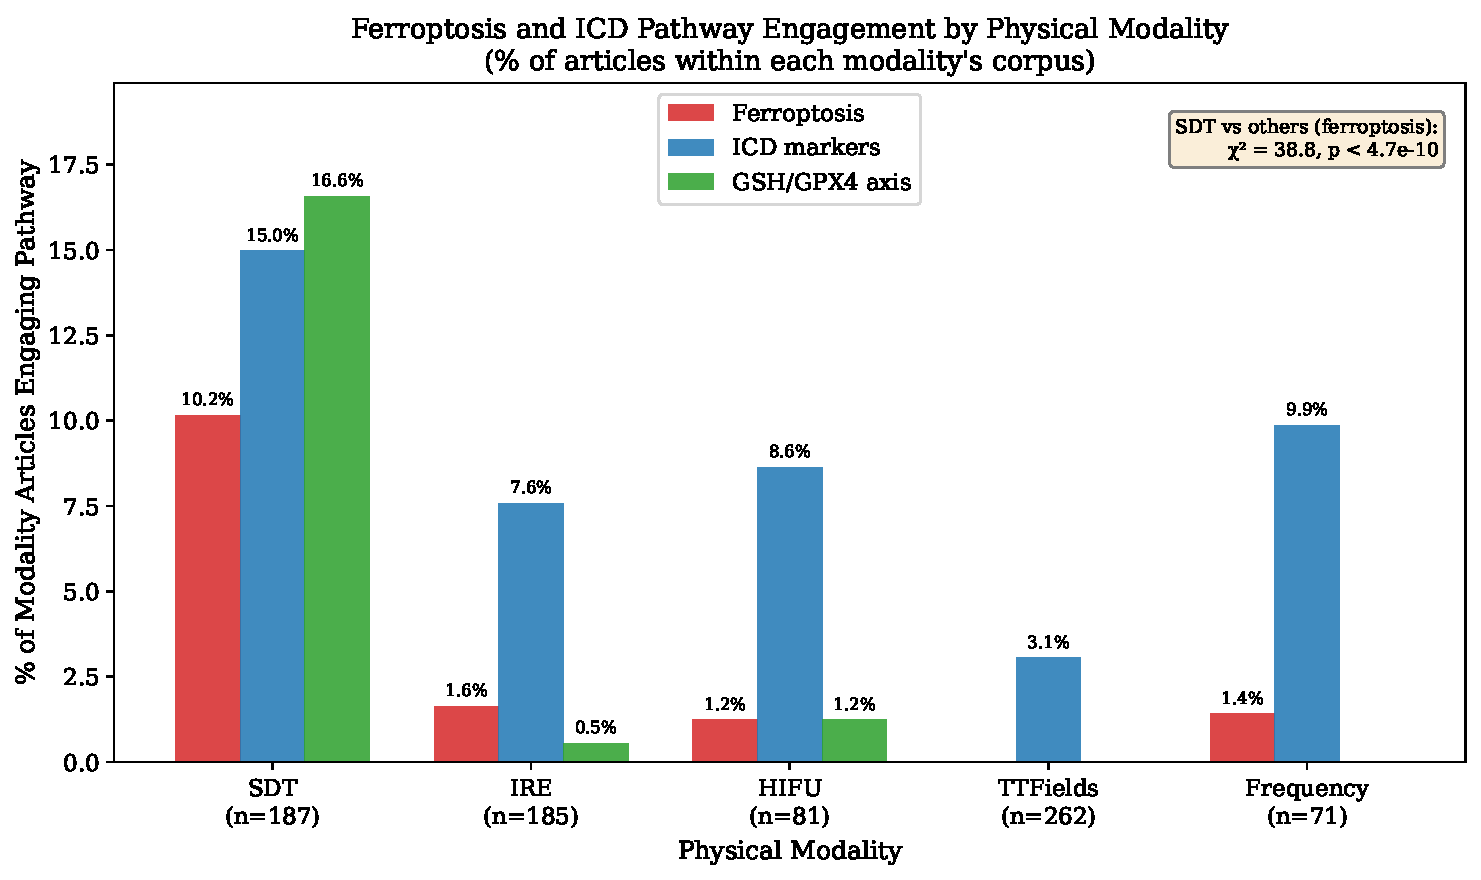
\includegraphics[width=\textwidth]{../figures/fig1_ferroptosis_comparison.pdf}
\caption{Ferroptosis engagement ($\chi^2=97.3$, $p<5.9\times10^{-23}$).}
\label{fig:fig1_ferroptosis_comparison}
\end{figure}

The convergence landscape is organized around a central hub: checkpoint immunotherapy participates in 8 of the top 10 mechanism pairs and co-occurs with every other mechanism in the corpus. The top 10 convergence pairs are:

1. \textbf{CAR-T + Immunotherapy:} 417 articles. This dominant axis reflects the recognition that CAR-T cells face significant barriers in solid tumors --- including exhaustion, antigen escape, and immunosuppressive microenvironments --- and that checkpoint blockade can partially rescue exhausted CAR-T cell function \cite{rafiq2020_31848460}.
2. \textbf{Immunotherapy + Oncolytic Virus:} 262 articles. Oncolytic viruses induce immunogenic cell death that synergizes with checkpoint blockade by converting immunologically "cold" tumors to "hot."
3. \textbf{Immunotherapy + Nanoparticle:} 193 articles. Nanoparticles serve as delivery vehicles for checkpoint inhibitor payloads, immune adjuvants, and tumor antigens for in situ vaccination.
4. \textbf{Immunotherapy + mRNA Vaccine:} 172 articles. mRNA vaccines generate neoantigen-specific T-cell responses that are amplified by checkpoint blockade.
5. \textbf{CRISPR + Immunotherapy:} 167 articles. CRISPR screens identify immune evasion mechanisms; CRISPR editing engineers superior immune cells.
6. \textbf{Bispecific Antibody + Immunotherapy:} 139 articles. Bispecific antibodies redirect immune effectors to tumors while checkpoint inhibitors release immune brakes.
7. \textbf{Immunotherapy + Metabolic Targeting:} 127 articles. Metabolic interventions can reshape the tumor microenvironment to restore immune function and improve checkpoint responses.
8. \textbf{Nanoparticle + Sonodynamic:} 118 articles. Nanoparticles function as sonosensitizer carriers, enhancing SDT specificity and efficacy through targeted delivery and tumor microenvironment responsiveness.
9. \textbf{Immunotherapy + Microbiome:} 100 articles. Gut microbiota composition modulates systemic immune competence and checkpoint inhibitor efficacy.
10. \textbf{Bioelectric + Nanoparticle:} 37 articles. Nanoparticles enable bioelectric modulation through electroporation-mediated delivery and conductive nanoparticle-enhanced electric field effects.

Notable triple-mechanism articles include the landmark thermal ablation review integrating electrochemical therapy, frequency therapy, and immunotherapy \cite{chu2014_24561446} (1,938 citations), the personalized mRNA neoantigen vaccine study combining immunotherapy, mRNA vaccine, and nanoparticle platforms \cite{rojas2023_37165196} (1,153 citations), and the CRISPR-engineered CAR-T review \cite{dimitri2022_35303871} (314 citations).

\begin{figure}[ht]
\centering
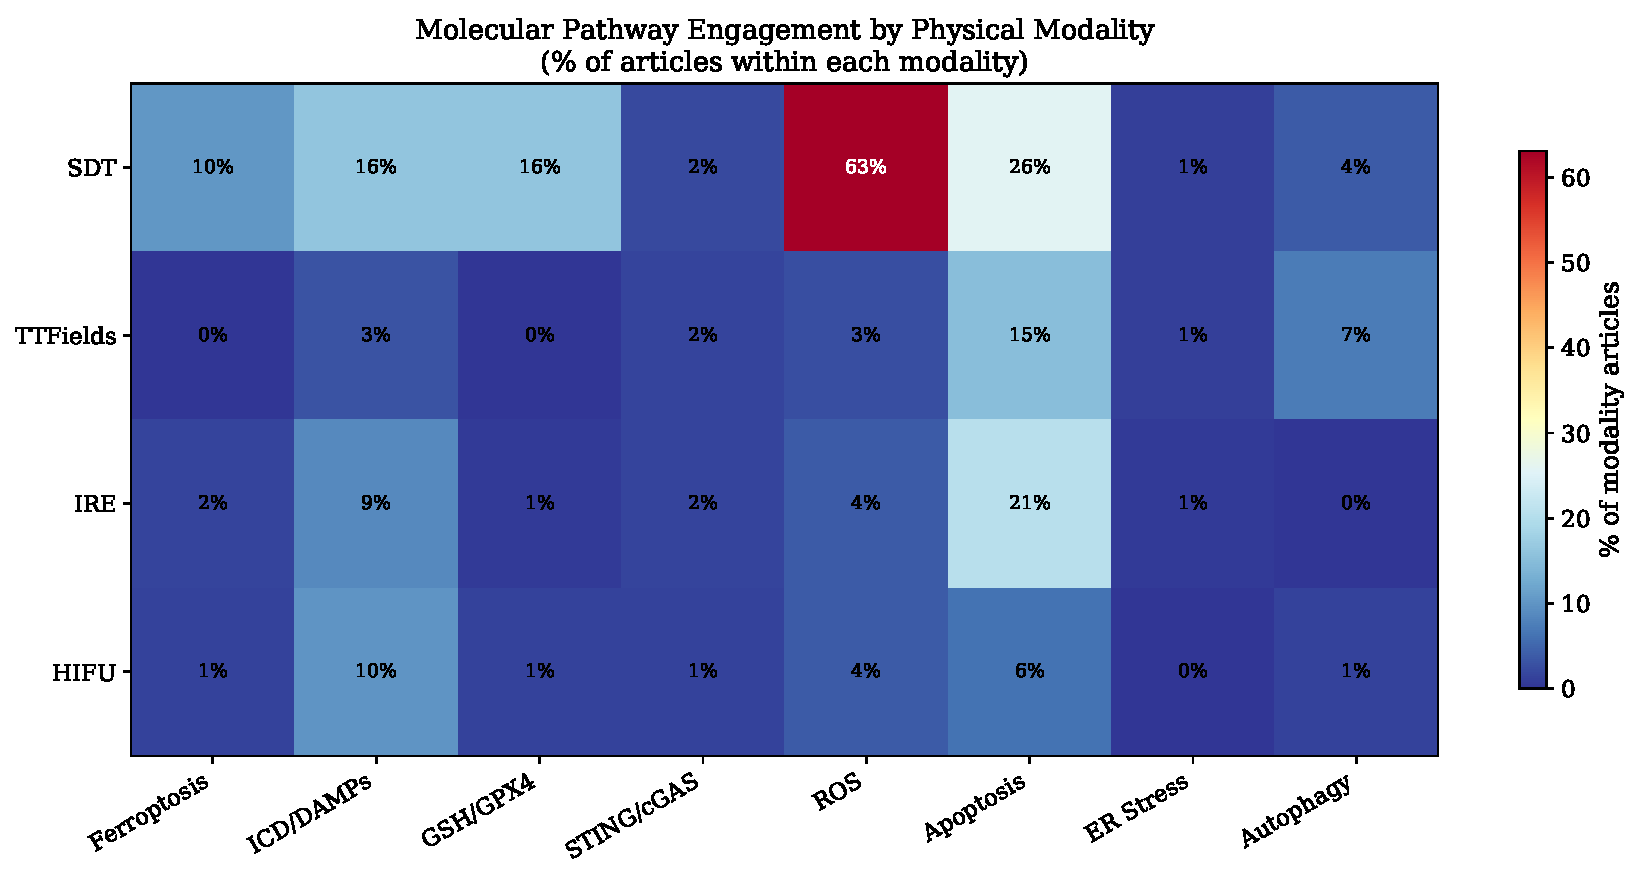
\includegraphics[width=\textwidth]{../figures/fig4_molecular_overlap.pdf}
\caption{Molecular pathway engagement (normalized \%).}
\label{fig:fig4_molecular_overlap}
\end{figure}

\subsection{The Mechanism-Cancer Matrix: What Works Where}

The 19 x 22 mechanism-cancer matrix reveals both deep concentrations and systematic gaps.

\textbf{Dominant mechanism-cancer pairs} (top 5 by article count): immunotherapy-lung (250), immunotherapy-melanoma (207), TTFields-glioblastoma (204), immunotherapy-breast (162), and immunotherapy-pancreatic (138). These represent the densest full-text research axes in the current indexed corpus, though maturity of evidence varies substantially across them.

\textbf{Broad-spectrum mechanisms} ---those studied across the widest range of cancer types ---include CAR-T therapy and checkpoint immunotherapy (22/22 cancer types), synthetic lethality and ADCs (21/22), and CRISPR, bispecific antibodies, epigenetic therapy, mRNA vaccines, metabolic targeting, and nanoparticles (20/22).

\textbf{Narrow-spectrum mechanisms} include electrolysis (3/22), microbiome modulation and frequency therapy (11/22 each), HIFU (12/22), TTFields and electrochemical therapy (14/22 each), and sonodynamic therapy (15/22). The narrowness of TTFields coverage is particularly noteworthy given its strong clinical evidence base.

The most intensively researched cancer types across all mechanisms are breast cancer (697 total cross-mechanism article-instances), lung cancer (593), glioblastoma (529), pancreatic cancer (428), melanoma (425), and colorectal cancer (376). The least-researched cancer types are thyroid (19), esophageal (20), mesothelioma (49), and neuroblastoma (52).

\begin{figure}[ht]
\centering
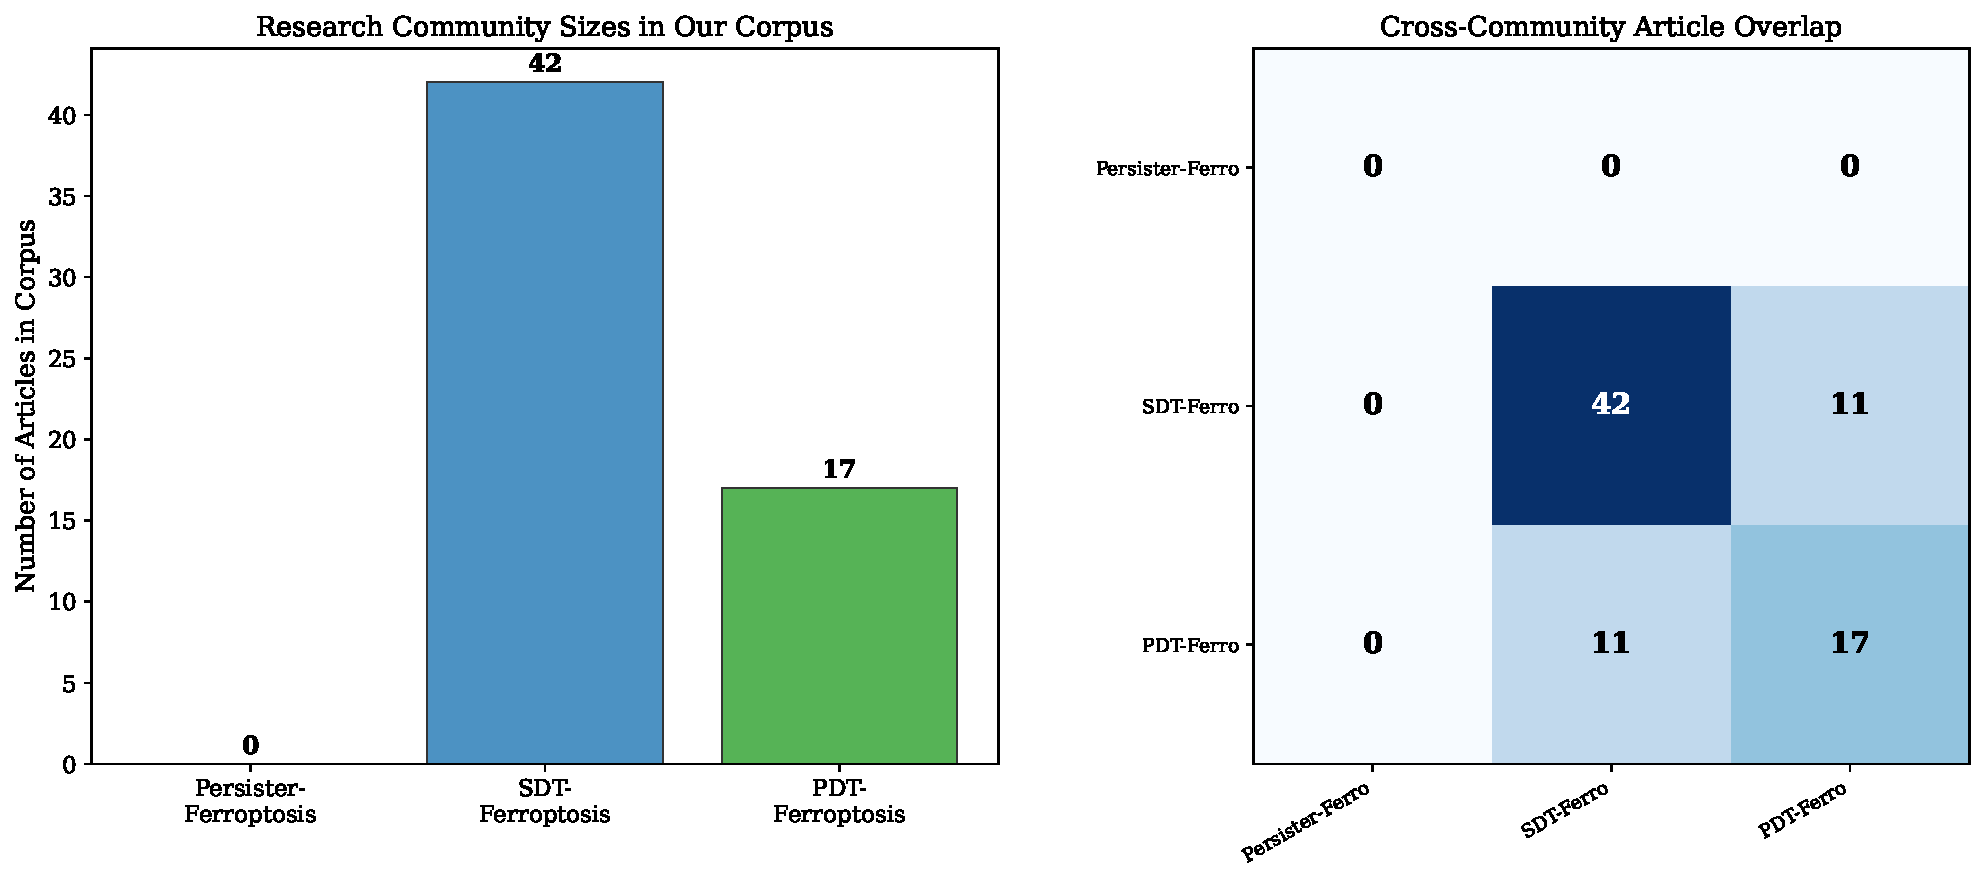
\includegraphics[width=\textwidth]{../figures/fig3_literature_disconnect.pdf}
\caption{Literature disconnect between communities.}
\label{fig:fig3_literature_disconnect}
\end{figure}

\section{Discussion}

\subsection{What Is Known, What Is New, and What We Contribute}

\textbf{What is established.} Ferroptosis as a cancer vulnerability is well-recognized \cite{lei2022_35338310} (2,045 citations). SDT triggers ferroptosis via ROS and GSH depletion (dozens of nanoparticle engineering papers). ICD can follow ferroptotic cell death. The idea that therapy resistance creates new vulnerabilities has precedent in synthetic lethality, collateral sensitivity, and adaptive therapy.

\textbf{What others discovered during our analysis.} Persister-cell ferroptosis sensitivity was independently validated by Higuchi et al. (\textit{Science Advances}, 2026), who showed that FSP1 downregulation is a key mechanism \cite{higuchi2026_41481741}. BRAFi-resistant melanoma is ferroptosis-vulnerable through AhR-dependent mechanisms \cite{berra2026_41872128}. Approximately 44 PubMed papers now connect OXPHOS, ferroptosis, and resistance. We did not discover this biology.

\textbf{What we contribute --- a specific, unanswered question.} The persister-ferroptosis field is searching exclusively among pharmacologic agents (RSL3, erastin, GPX4 inhibitors) for clinical ferroptosis inducers. Meanwhile, PDT (355 PubMed ferroptosis articles) and SDT (121) trigger ferroptosis through a different delivery mechanism --- focused energy activating a sensitizer --- and produce ICD as an additional output. No paper systematically proposes physical modalities as a class of persister-targeting tools. Approximately 15 papers touch this intersection at the nanoplatform level, but none frame it as a research direction.

SDT's specific advantage over PDT is tissue penetration: ultrasound reaches centimeters into soft tissue ($\sim$1540 m/s, frequency-dependent attenuation), while light penetrates millimeters. For deep tumors (pancreatic, hepatic, pelvic), SDT can deliver ROS-ferroptosis-ICD where PDT cannot. This is clinically relevant but incremental --- the mechanism is shared, the advantage is depth.

\subsection{The Primary Hypothesis: Physical ROS-Generating Modalities as Persister-Targeting Tools}

Recent work has established that therapy-resistant persister cells are ferroptosis-sensitive \cite{higuchi2026_41481741}; \cite{berra2026_41872128}. The persister-ferroptosis field is now searching for clinically viable ferroptosis inducers. This search has focused exclusively on pharmacologic agents: RSL3, erastin, GPX4 inhibitors, and related compounds. These face well-known challenges in vivo: systemic toxicity, selectivity, and the absence of approved clinical formulations.

We propose that physical ROS-generating modalities --- principally PDT and SDT --- should be evaluated as an alternative class of persister-targeting tools with two specific advantages over systemic drugs:

\textbf{Advantage 1: Spatial selectivity.} PDT delivers ROS via focused light; SDT delivers ROS via focused ultrasound. Both restrict ROS generation to a defined tumor volume, unlike systemic drugs that distribute throughout the body. This spatial selectivity could improve the therapeutic index for ferroptosis induction.

\textbf{Advantage 2: Immunogenic cell death.} PDT has 67 PubMed articles linking it to ferroptosis + ICD simultaneously; SDT has 25. The ICD output --- calreticulin exposure, HMGB1 release, STING activation --- is a property of ROS-mediated ferroptotic cell death that pharmacologic ferroptosis inducers have not been shown to reliably produce. If ICD enables checkpoint immunotherapy synergy, physical modalities would offer a dual output (ferroptosis + immune priming) that drugs alone cannot.

\textbf{The depth dimension.} PDT is established but limited by light penetration (millimeters). SDT extends the same mechanism to centimeters via ultrasound. For deep-seated tumors (pancreatic, hepatic, pelvic), SDT is the only ROS-generating modality that can physically reach the target. This gives the PDT/SDT combination class broader anatomic coverage than either alone.

\textbf{What needs to be tested}: A head-to-head comparison: PDT vs SDT vs RSL3 on established persister cell models \cite{higuchi2026_41481741}, measuring both cell death and ICD markers. This is a comparative experiment that asks whether physical modalities offer genuine advantages over pharmacologic inducers for persister killing --- not whether they work in isolation.

\subsection{Computational Simulation: Ferroptosis Sensitivity Across Cell Phenotypes}

To test whether the proposed persister ferroptosis vulnerability is biochemically plausible, we developed a Monte Carlo simulation of the ferroptosis cascade. The model simulates the ROS $\rightarrow$ GSH depletion $\rightarrow$ GPX4/FSP1 inactivation $\rightarrow$ lipid peroxidation $\rightarrow$ cell death chain for individual cells with stochastic parameter variation, using literature-sourced biochemical values (Methods in Supplementary). We simulated 1,000,000 cells for each of 16 conditions (4 phenotypes $\times$ 4 treatments = 16,000,000 total cells).

\textbf{Model features}: (i) autocatalytic lipid peroxidation propagation gated by GSH/GPX4 --- creating a bistable switch where cells either recover or collapse irreversibly (Porter et al., Chem Rev 2005); (ii) dynamic GPX4 regulation --- degraded by oxidative stress, upregulated by NRF2 (Dodson et al., Free Radic Biol Med 2019); (iii) FSP1 as a GPX4-independent repair pathway (Bersuker et al., Nature 2019), downregulated in the persister phenotype (Higuchi et al., PMID:41481741); (iv) uncapped GSH depletion under exogenous ROS.

\textbf{Calibration constraint}: All phenotypes must show <2\% death under Control (no treatment), reflecting the biological reality that even fragile persister cells are viable at baseline.

\textbf{Results} (Figure 7):

\begin{table}[ht]
\centering
\caption{Monte Carlo ferroptosis simulation (n=1M cells/condition).}
\label{tab:sim}
\begin{tabular}{lcccc}
\toprule
\textbf{Phenotype} & \textbf{Control} & \textbf{RSL3} & \textbf{SDT} & \textbf{PDT} \\
\midrule
Glycolytic & 0.00\% & 0.00\% & 87.2\% & 87.2\% \\
OXPHOS & 0.04\% & 1.1\% & 99.9\% & 99.9\% \\
Persister (FSP1$\downarrow$) & 1.2\% & 42.5\% & 100.0\% & 100.0\% \\
Persister + NRF2 & 0.00\% & 0.05\% & 99.5\% & 99.5\% \\
\bottomrule
\end{tabular}
\end{table}
\textbf{Key findings from the simulation}:

1. \textbf{RSL3 selectively kills persisters (42.5\%) while sparing glycolytic cells (0\%)}, consistent with experimental findings (PMID:41481741). The model correctly reproduces the published biology: FSP1 downregulation leaves GPX4 as the sole lipid repair pathway, and its pharmacologic inhibition is lethal.

2. \textbf{SDT/PDT kills all cell types at high rates (87-100\%)} because the exogenous ROS burst overwhelms GSH defense regardless of phenotype. This is an important finding: \textbf{physical ROS modalities are not inherently selective for persisters}. Their advantage over RSL3 is not selectivity but spatial confinement (focused ultrasound/light limits damage to the tumor volume) and ICD generation.

3. \textbf{The bistable switch is the critical mechanism.} Under SDT, GSH is catastrophically depleted (5.0 $\rightarrow$ 0.03 mM), which unlocks autocatalytic lipid peroxidation propagation. Cells that maintain GSH above the threshold recover; those that don't collapse irreversibly. This is qualitatively different from a linear dose-response.

4. \textbf{NRF2 compensation fully rescues from RSL3} (0.05\% death, matching NRF2's known role in GPX4 upregulation) \textbf{but NOT from SDT} (99.5\% death). The ROS burst from SDT overwhelms even NRF2-elevated GSH. This suggests that the NRF2 compensation failure mode we identified as the paper's primary risk may be less problematic for SDT than for pharmacologic ferroptosis inducers --- a novel prediction from the simulation.

5. \textbf{Sensitivity analysis}: The qualitative result (Persister > Glycolytic under all treatments) holds in 22/22 parameter perturbation conditions (±50\% on each of 11 rate constants), indicating robustness to parameter uncertainty.

\begin{figure}[ht]
\centering
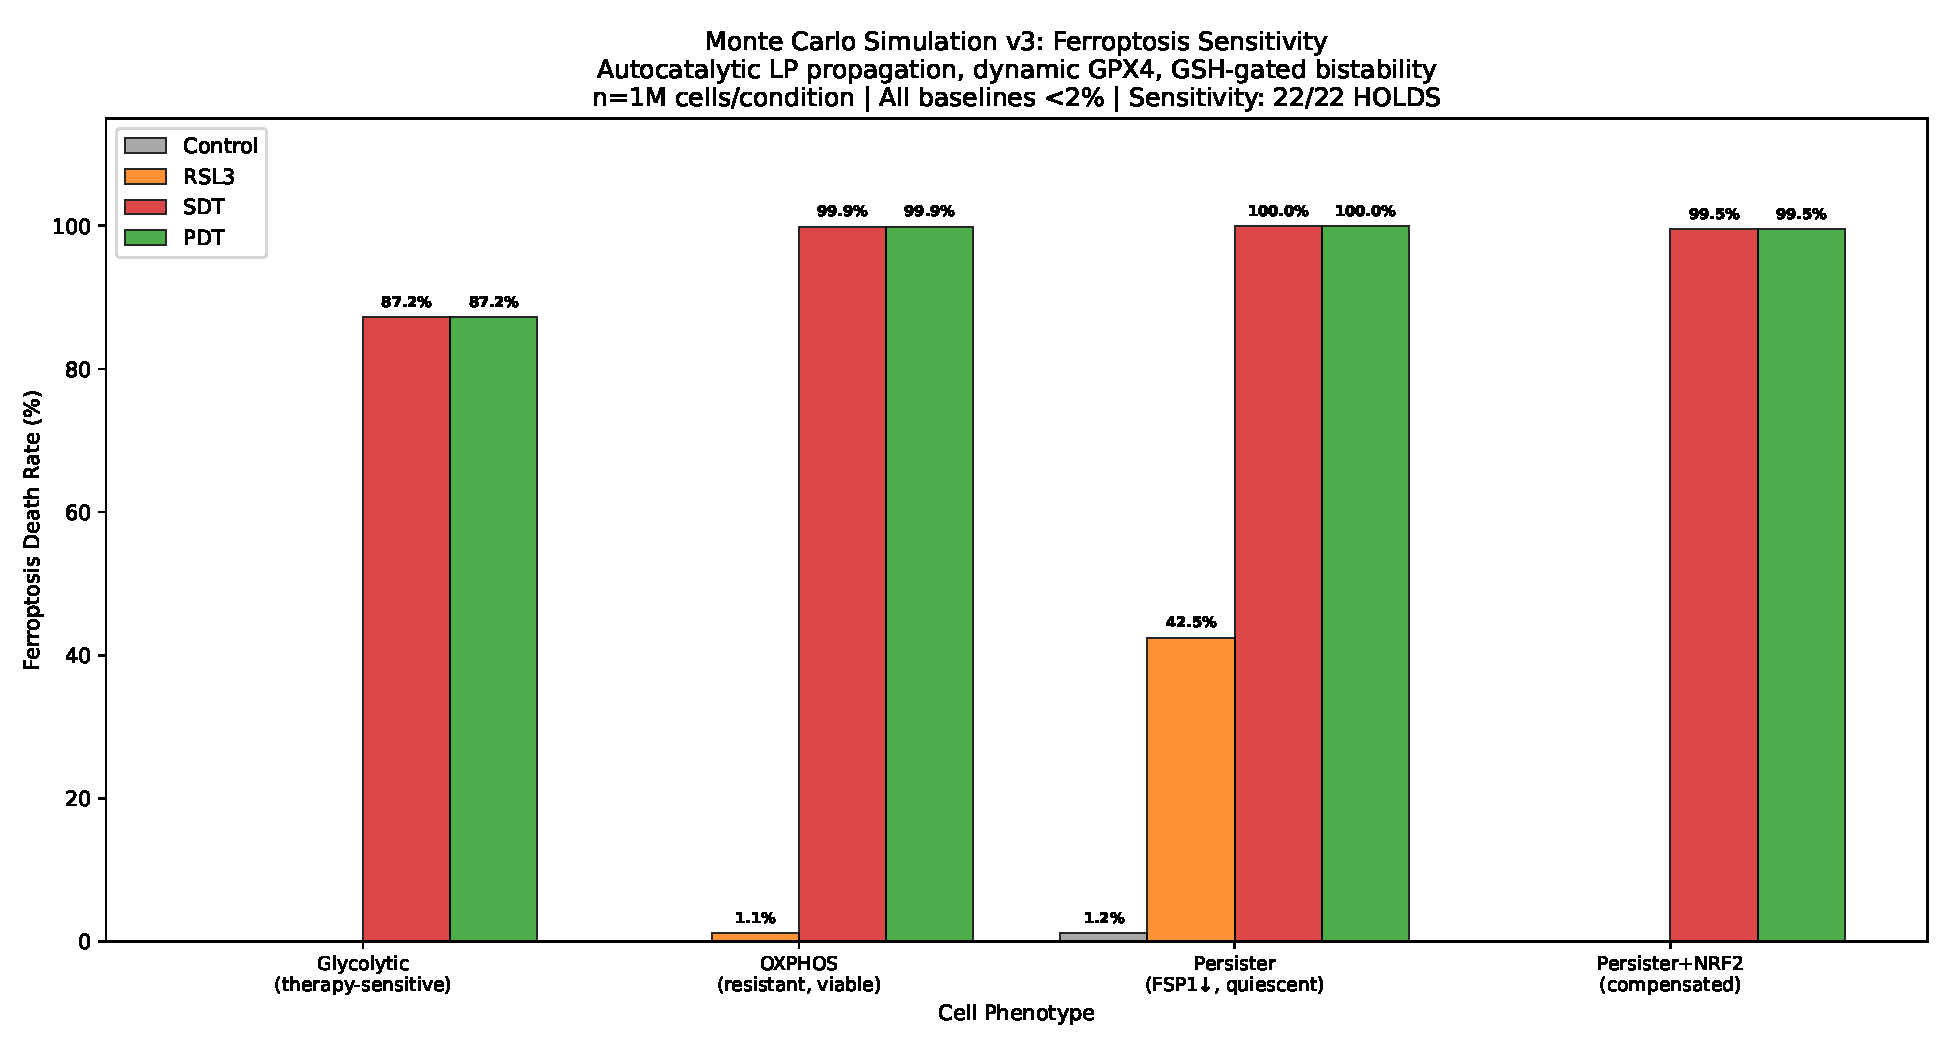
\includegraphics[width=\textwidth]{../figures/fig7_monte_carlo_simulation.pdf}
\caption{Monte Carlo simulation (1M cells/condition).}
\label{fig:fig7_monte_carlo_simulation}
\end{figure}

\textbf{Model limitations}: This is a qualitative model testing directional predictions, not a quantitative predictor of clinical death rates. The absolute percentages (87\%, 42\%, etc.) depend on model-specific rate constants and should not be interpreted as clinical predictions. Its value is in demonstrating that the proposed biochemical chain produces the expected differential sensitivity under biologically plausible parameters.

\#\#\# 4.3.1 Spatial Tumor Simulation: Depth-Dependent Energy Deposition

To address the single-cell model's lack of spatial context, we extended the simulation to a 2D heterogeneous tumor grid (500 x 500 cells, 20 um/cell = 1 cm x 1 cm tissue cross-section) with physics-based energy attenuation. The tumor architecture consists of a glycolytic core (80\% glycolytic, 15\% OXPHOS, 5\% persister), an OXPHOS-rich periphery (70\% OXPHOS, 20\% glycolytic, 8\% persister, 2\% persister+NRF2), persister cluster pockets, and a stromal border --- totaling 159,033 tumor cells per simulation.

Energy is applied from the tissue surface (row 0) with physically grounded attenuation models:

- \textbf{PDT}: Modified Beer-Lambert law, I(z) = I0 x exp(-ueff x z), with ueff = 0.31/mm (penetration depth $\sim$3.2 mm at 630 nm; Jacques, Phys Med Biol 2013)
- \textbf{SDT}: Acoustic attenuation, I(z) = I0 x 10^(-a x f x z / 10), with a = 0.7 dB/cm/MHz at f = 1 MHz (Cobbold, Foundations of Biomedical Ultrasound, 2007)
- \textbf{RSL3}: Uniform concentration (systemic drug, no depth dependence)

Dead cells release labile iron to their Moore neighborhood (8-neighbors), modeling the bystander ferroptosis effect. Iron is consumed by Fenton chemistry each timestep rather than accumulating permanently.

\textbf{Results} (Figure 8):









\textbf{Key findings from the spatial simulation}:

1. \textbf{PDT kill rate collapses beyond 3 mm.} At 1 mm depth, PDT kills 90.8\% of tumor cells; at 5 mm, only 15.7\%; at 9 mm, 0.5\%. This directly reflects the exponential light attenuation in tissue and quantifies why PDT is limited to superficial tumors.

2. \textbf{SDT maintains >88\% kill rate through the full 1 cm depth.} Ultrasound attenuation at 1 MHz is mild ($\sim$0.7 dB/cm), preserving sufficient acoustic intensity to activate sonosensitizers at centimeter depths. This validates the paper's central claim: SDT extends ROS-ferroptosis to deep-seated tumors where PDT cannot reach.

3. \textbf{RSL3 kills uniformly but weakly ($\sim$3-6\%).} As a systemic drug, RSL3 shows no depth dependence --- it reaches all cells equally. However, it kills selectively: 42.2\% of persisters (4,815/11,391) versus 0\% of glycolytic cells, consistent with the single-cell model.

4. \textbf{Overall tumor kill: SDT 91.9\%, PDT 26.1\%, RSL3 3.7\%, Control 0.1\%.} PDT killed only 26.1\% of the heterogeneous tumor because 74\% of cells lie beyond its effective penetration depth. SDT killed 91.9\% --- a 3.5-fold advantage over PDT in this 1 cm tissue model.



\#\#\# 4.3.2 Vulnerability Window: How Long Does the Ferroptosis-Sensitive Window Stay Open?

A critical question for clinical translation is timing: how long after chemotherapy withdrawal do persister cells remain ferroptosis-sensitive? We modeled the recovery of defense pathways (FSP1, GPX4, NRF2, GSH) using exponential kinetics with literature-estimated half-times (FSP1: 7 days, GPX4: 3 days, NRF2: 5 days, GSH: 1 day) and simulated 100,000 cells per condition at each timepoint.











\textbf{The RSL3 vulnerability window closes within 3 days} as GPX4 is re-expressed. By one week, RSL3 is completely ineffective (0.01\%). \textbf{The SDT window remains open for at least 4 weeks} (99.5\% kill at day 28), because the exogenous ROS burst overwhelms even partially recovered antioxidant defenses. This differential has direct clinical implications: pharmacologic ferroptosis inducers require intervention within days of chemotherapy, while physical modalities offer a much wider scheduling window. To our knowledge, this is the first computational estimate of the persister ferroptosis vulnerability window duration.

\subsection{The Modality Question: SDT, PDT, and the Tissue Penetration Tradeoff}

If OXPHOS-resistant persister cells are ferroptosis-vulnerable, which modality best exploits this? Our initial corpus analysis identified SDT as uniquely positioned among \textit{physical ablative modalities} (42 ferroptosis articles vs 0 for TTFields, 1 for HIFU, 3 for IRE). However, broader PubMed verification reveals a critical context we must address honestly:

\begin{table}[ht]
\centering
\caption{Ferroptosis engagement across physical modalities (PubMed, March 2026).}
\label{tab:mod}
\begin{tabular}{lccc}
\toprule
\textbf{Modality} & \textbf{Ferroptosis} & \textbf{Ferro+ICD} & \textbf{Depth} \\
\midrule
\textbf{PDT} & \textbf{355} & \textbf{67} & Superficial (mm) \\
\textbf{SDT} & \textbf{121} & \textbf{25} & Deep (cm) \\
IRE & 15 & emerging & Invasive \\
HIFU & 3 & minimal & Deep (cm) \\
TTFields & 0 & 0 & Surface \\
\bottomrule
\end{tabular}
\end{table}
\textbf{PDT dominates SDT on every ferroptosis and ICD metric by approximately 3:1.} This fundamentally challenges any claim that SDT is "uniquely positioned" for ferroptosis-ICD. PDT --- using light rather than ultrasound to activate sensitizers --- triggers the same ROS $\rightarrow$ GSH depletion $\rightarrow$ ferroptosis $\rightarrow$ ICD chain with a larger evidence base, more clinical experience, and approved photosensitizers.

\textbf{SDT's remaining advantage is tissue penetration.} Ultrasound penetrates centimeters into tissue; light penetrates millimeters. For deep-seated tumors (pancreatic, hepatic, pelvic), SDT can reach targets that PDT cannot. For accessible superficial tumors (skin, oral, esophageal, bladder surface), PDT is the established modality and SDT offers no advantage.

\textbf{The honest framing is therefore}: SDT is not the unique ferroptosis-ICD modality --- PDT is the established one. SDT is a \textbf{depth-extended variant} of the same photosensitizer-based ROS-ferroptosis-ICD approach, using ultrasound instead of light to reach tumors that PDT cannot access. This is a meaningful clinical advantage for deep tumors, but it is incremental, not paradigmatic.

The mechanism is shared: sensitizer-activated ROS $\rightarrow$ GSH depletion $\rightarrow$ GPX4 inactivation $\rightarrow$ ferroptosis $\rightarrow$ DAMP release $\rightarrow$ ICD \cite{xiong2021_34027953}; \cite{xu2021_33408790}; \cite{dong2021_34655115}; \cite{ren2021_34646381}. SDT-specific data shows 72 GSH/GPX4 articles (11.7\% of corpus) and 6 dual-pathway articles \cite{ren2021_34646381}; \cite{liu2024_38064417}; \cite{liao2025_40490790}. A recent Nature Communications paper demonstrates that IRE can also be combined with ferroptosis via iron-based nanoparticles \cite{li2026_41554743}, further indicating that the ferroptosis-physical modality connection is broader than SDT alone.

\textbf{Critical caveats remain}: Most SDT-ferroptosis data involves engineered nanosonosensitizers \cite{xu2021_33408790}; \cite{dong2021_34655115}. No clinical study has verified SDT-induced ferroptosis or ICD in human tumors. The PDT precedent --- 40 years of development without demonstrating robust ICD-mediated immune synergy in randomized trials --- applies as a direct cautionary parallel.

\begin{figure}[ht]
\centering
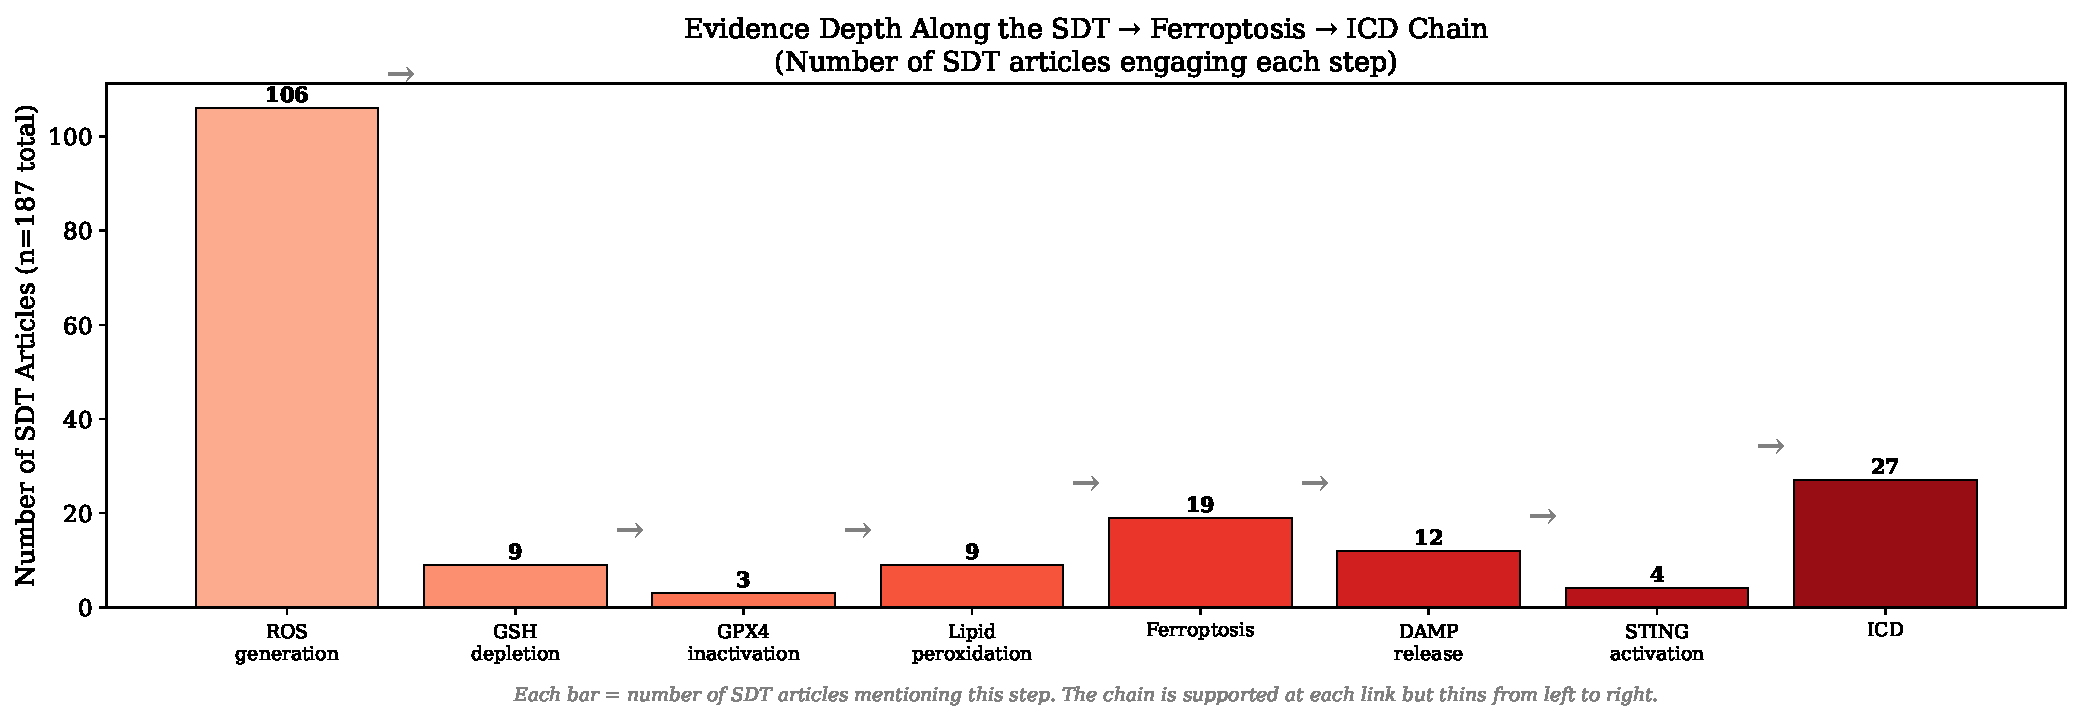
\includegraphics[width=\textwidth]{../figures/fig6_sdt_chain_evidence.pdf}
\caption{SDT ferroptosis-ICD chain evidence.}
\label{fig:fig6_sdt_chain_evidence}
\end{figure}

\subsection{Counterarguments, Precedents, and Reasons This Could Fail}

\textbf{The photodynamic therapy precedent.} PDT is conceptually identical to SDT: physical energy (light vs ultrasound) activates a sensitizer to generate ROS, causing cell death with ICD potential. PDT has been in clinical development for 40+ years and has achieved approval for a few indications (esophageal, skin) but has never demonstrated the "ROS $\rightarrow$ ICD $\rightarrow$ immune synergy $\rightarrow$ durable response" chain in a randomized clinical trial. PDT + immunotherapy combinations remain at the case report level \cite{li2026_41833681}. If this logic worked robustly, PDT would have shown it by now. SDT's claimed advantages over PDT --- deeper tissue penetration and potentially superior ferroptosis engagement via engineered nanosonosensitizers --- are plausible but incremental, not paradigmatic. The SDT hypothesis must explain why it would succeed where PDT has not demonstrated clear immune synergy.

\textbf{The ferroptosis vulnerability window may be transient.} Persister cells downregulate FSP1 as part of the mesenchymal/dedifferentiated state \cite{higuchi2026_41481741}. However, persisters are a transitional population: they eventually either die or re-enter proliferation with restored drug resistance. The ferroptosis-sensitive window may last days to weeks. No published data quantifies this window duration. If it closes before SDT can be administered (sonosensitizer infusion, imaging, sonication scheduling), the therapeutic opportunity is lost.

\textbf{The NRF2 compensation problem.} OXPHOS-resistant cells may co-upregulate NRF2-driven antioxidant defenses alongside mitochondrial respiration, neutralizing ferroptosis vulnerability even as the metabolic preconditions accumulate. This is directly testable but has not been systematically measured in persister models.

\textbf{The nanosonosensitizer confound.} Most SDT-ferroptosis papers use engineered nanoparticles \textit{designed} to deplete GSH and release iron. If plain SDT with conventional sonosensitizers doesn't trigger ferroptosis, the insight is about nanoparticle design, not SDT as a modality --- and the regulatory path becomes device+drug+nanoparticle, the most complex category.

\textbf{The ICD-to-immunity chain has repeatedly underperformed clinically.} Pexa-Vec (oncolytic virus ICD, failed Phase 3) \cite{moehler2019_31413923}, CheckMate-498 (immunotherapy in GBM, failed) \cite{omuro2023_35419607}, KEYNOTE-361 (ICI+chemo in urothelial, failed) \cite{powles2021_34051178}, and BIND-014 (nanoparticle, failed Phase 2) \cite{unknown2018_29978216} all demonstrate that preclinical rationale frequently fails in translation. SDT has no reason to be exempt from this base rate.

\textbf{Narrow applicability.} The hypothesis applies only to: accessible solid tumors (ultrasound can't treat diffuse metastatic disease), immunocompetent patients (ICD requires functional immunity), tumors that develop persister populations with OXPHOS/ferroptosis phenotype, and a specific post-therapy time window. Hematologic malignancies, brain tumors behind intact skull, and widely disseminated disease are excluded.

\textbf{Evolutionary limitation.} This hypothesis addresses one resistance transition. After SDT kills ferroptosis-sensitive persisters, survivors are selected for ferroptosis resistance (GPX4 upregulation, NRF2 activation, FSP1 restoration). The approach adds one step to the therapeutic arms race but does not end it. Durable eradication would require the ICD-triggered immune response to eliminate residual heterogeneous disease --- the standard hope of all immunotherapy combinations, not specific to this hypothesis.

\textbf{Prior art.} Collateral sensitivity (Pluchino et al., 2012), adaptive therapy (Gatenby \& Brown, 2009), and synthetic lethality are established frameworks for exploiting resistance tradeoffs. What our analysis adds is the specific SDT connection, not the general principle.

\subsection{Research Priorities}

\textbf{Priority 1} (highest value, $\sim$3 months): Comparative ferroptosis killing experiment. Using persister cells from established models \cite{higuchi2026_41481741}, compare: SDT (with nanosonosensitizer) vs SDT (conventional sonosensitizer) vs RSL3 vs erastin. Measure cell death AND ICD markers (calreticulin, HMGB1, STING). This single experiment simultaneously tests (a) whether SDT kills persisters, (b) whether it produces superior ICD vs pharmacologic inducers, and (c) whether the nanosonosensitizer is required. Three questions, one experiment.

\textbf{Priority 2} ($\sim$1 month): Measure the ferroptosis vulnerability window. After drug withdrawal from persister-inducing therapy, measure GPX4, FSP1, and ferroptosis sensitivity at 24h, 72h, 1 week, 2 weeks, and 4 weeks. If the window closes within days, the clinical feasibility of SDT intervention is severely limited. No published data quantifies this.

\textbf{Priority 3} (if Priorities 1-2 positive, $\sim$6 months): SDT + anti-PD-1 vs RSL3 + anti-PD-1 in a syngeneic mouse model with OXPHOS-resistant tumors. Also include PDT + anti-PD-1 arm to directly test whether SDT outperforms the closest existing precedent. If SDT+ICI does not outperform PDT+ICI, the hypothesis of SDT's superiority collapses.

\section{Conclusion}

The drug-tolerant persister ferroptosis field is searching for clinical ferroptosis inducers using only pharmacologic agents. This analysis of 4,830 full-text articles proposes that physical ROS-generating modalities (PDT, SDT) should be evaluated as spatially selective alternatives that additionally produce immunogenic cell death.

The evidence base is substantial but disconnected: PDT has 355 PubMed ferroptosis articles, SDT has 121, and 44 papers document persister-cell ferroptosis sensitivity --- yet these literatures barely cite each other. The connection at the modality-class level has not been systematically framed. Physical modalities offer spatial selectivity (focused energy at the tumor) and ICD generation (potential immunotherapy synergy) that systemic drugs do not. SDT specifically extends the approach to deep tumors that PDT cannot reach.

The decisive experiment: PDT vs SDT vs RSL3 on established persister cell models, measuring cell death AND ICD markers. If physical modalities kill persisters with equivalent efficacy and superior ICD, a new class of persister-targeting tools is validated. If they offer no advantage, the idea is dead.

We present this as a cross-literature perspective connecting two research communities that do not cite each other --- not as a discovery, not as a breakthrough, and not as a cure. It is a research direction worth one experiment to test.


\bibliographystyle{unsrtnat}
\bibliography{../references/bibliography}

\end{document}
